\section{Nền tảng lý thuyết}
\subsection{Ikigai}
\textbf{Ikigai} là một khái niệm đến từ văn hóa Nhật Bản, mang ý nghĩa là “lý do để sống” hoặc “lý do để thức dậy vào buổi sáng”. Đây không chỉ là một từ ngữ, mà còn là một triết lý sống, một cách tiếp cận cuộc sống hàng ngày với niềm đam mê, sự hài lòng và một cảm giác rằng mình đang làm những điều có ý nghĩa. Ikigai được cho là có liên quan mật thiết đến hạnh phúc và tuổi thọ lâu dài.Nói một cách đơn giản, Ikigai là lý do bạn thức dậy vào mỗi buổi sáng. Với rất nhiều người, tiếng chuông báo thức là thứ buộc họ tỉnh giấc vào mỗi buổi sáng, nhưng chính niềm vui mà chúng ta kỳ vọng sẽ diễn ra trong ngày mới là điều thôi thúc ta rời khỏi giường. Và với người Nhật, Ikigai là niềm vui ấy. Tuy vậy Ikigai trở thành một đề tài khó diễn giải, ngay cả đối với người Nhật, là mặc dù khái niệm này rất phổ biến ở Nhật, nhưng nó không có trong sách vở. Theo Yukari Mitsuhashi, tác giả của cuốn “Ikigai - chất Nhật trong từng khoảnh khắc” từng chia sẻ“ Tôi trưởng thành và sống phần lớn cuộc đời mình tại Nhật, nhưng tôi không nhớ trường học từng dạy tôi về Ikigai.”. Chỉ riêng cấp tiểu học, học sinh Nhật Bản đã học hơn 1.000 chữ kanji, nhưng trong số đó không có Ikigai.6 Nó là từ phổ biến đến nỗi mọi người thoải mái dùng hằng ngày mà chẳng hề quan tâm nó có ý nghĩa gì đặc biệt hay không. Ikigai là một khái niệm đa diện mà chúng ta sẽ dần hiểu ra trong quá trình sống và trưởng thành. “Ikigai của bạn là gì?” không phải là một câu hỏi đơn giản với một đáp án duy nhất, mà là một câu hỏi trừu tượng với vô số câu trả lời khả dĩ. Trong trường nghĩa này, nó là một khái niệm rộng miêu tả đa dạng những khía cạnh khác
nhau của cuộc sống. Đúng là Ikigai có thể mang lại thành công, nhưng thành công
không phải là một điều kiện tất yếu để có Ikigai. Quan trọng nhất không hẳn là phải
thành công trong sự nghiệp mà là bạn có thể đạt được Ikigai không. Chính điều thôi
thúc bạn thức dậy vào mỗi buổi sáng mới chính là Ikigai của bạn - và không ai có thể
nói bạn hãy chọn đáp án khác. Có thể nói đó là ý niệm cơ bản nhất về Ikigai trong tiềm
thức của mỗi người Nhật.

Khái niệm Ikigai, với ý nghĩa là "lý do tồn tại" trong tiếng Nhật, mang tính trừu tượng cao, làm cho việc xác định Ikigai trở thành một thách thức đối với nhiều người, bao gồm cả bản thân mỗi người. Để giúp làm rõ hơn và hỗ trợ quá trình này, sơ đồ Ikigai Venn đã ra đời, nguồn gốc của sơ đồ bắt nguồn từ chiêm tinh gia người Tây Ban Nha, Andres Zuzunaga. Cấu trúc này được giới thiệu lần đầu tiên trong cuốn sách \textit{"Qué Harías Si No Tuvieras Miedo"} (Tạm dịch: Bạn sẽ làm gì nếu bạn không sợ?) của tác giả Borja Vilaseca. Sơ đồ Venn đã trở nên nổi tiếng và được nhiều người hiểu nhầm là khái niệm Ikigai của Nhật Bản. Sơ đồ này, được gọi là “Purpose Venn Diagram” hay “Cosmograma”, được tạo ra để giúp mọi người tìm ra mục đích sống của họ bằng cách xác định điều gì họ yêu thích, điều gì họ giỏi, điều gì thế giới cần, và điều gì họ có thể kiếm tiền từ đó. Zuzunaga tin rằng sơ đồ của ông kết nối với tâm lý học, khoa học, xã hội và triết học, và nhấn mạnh tầm quan trọng của việc tự phản ánh và suy ngẫm về mục đích sống của bản thân. Ông cho rằng việc tập trung vào sự biến đổi nội tâm là quan trọng hơn các hoàn cảnh bên ngoài, vì nó cho phép cá nhân khám phá bản thực của mình và đóng góp tiềm năng của họ cho thế giới.

\begin{figure}[H]
    \centering
    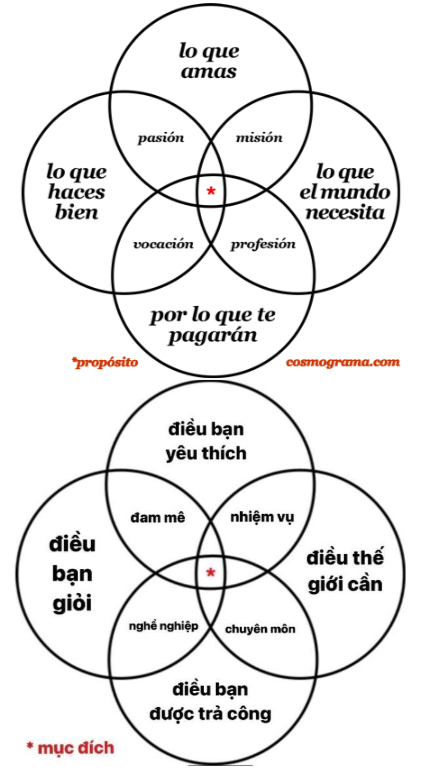
\includegraphics[width=0.5\linewidth]{images/zuzunaga.png}
    \vspace{0.6cm}
    \caption{Sơ đồ Venn mục đích của Zuzunaga}
\end{figure}

Sơ đồ Venn Ikigai, là một công cụ hình ảnh giúp mọi người xác định “lý do tồn tại” của mình bằng cách tìm ra điểm giao thoa giữa những gì họ yêu thích, những gì họ giỏi, những gì thế giới cần và những gì họ có thể kiếm tiền từ đó. Được tạo ra bởi doanh nhân người Mỹ Marc Winn, người đã kết hợp “Sơ đồ Venn Mục Đích” của Andrés Zuzunaga với khái niệm Ikigai của Nhật Bản. Sơ đồ Ikigai Venn được cấu trúc dựa trên bốn yếu tố chính:

\begin{itemize}
    \item Đam mê (What you love): Điều bạn yêu thích làm, những hoạt động khiến bạn cảm thấy hạnh phúc và thỏa mãn.
    \item Nghề nghiệp (What you are good at): Những kỹ năng và tài năng mà bạn có, những công việc mà bạn thực hiện tốt.
    \item Nhu cầu của thế giới (What the world needs): Những đóng góp mà bạn có thể mang lại cho xã hội, những nhu cầu mà thế giới đang cần đến.
    \item Nghề nghiệp có thể kiếm tiền (What you can be paid for): Những công việc mà bạn có thể nhận được sự đền đáp về mặt tài chính. 
\end{itemize}

Sơ đồ Ikigai Venn của Marc Winn đã giúp định hình lại cách mà nhiều người nhìn nhận về việc tìm kiếm mục đích sống. Trước khi sơ đồ này được tạo ra, khái niệm Ikigai thường được cảm nhận thông qua trải nghiệm sống hoặc được mô tả bằng những ví dụ thực tế về đam mê của mọi người. Tuy vậy, không có hình ảnh cụ thể nào được liên kết với Ikigai cho đến khi Marc Winn tạo ra sơ đồ này. Marc Winn đã viết một bài đăng blog vào năm 2014, giới thiệu sơ đồ Ikigai Venn\footnote{Marc Winn, \textit{"What is your Ikigai?"}, từ https://theviewinside.me/what-is-your-Ikigai, truy cập ngày: 14.05.2014)}. Ông đã lấy cảm hứng từ công việc của Dan Buettner về các “Blue Zones” - những khu vực trên thế giới có tỷ lệ người sống thọ cao. Cụ thể, bài nói chuyện TED của Dan Buettner với tiêu đề “Làm thế nào để sống đến 100 tuổi” đã đề cập đến khái niệm Ikigai. Kết hợp ý tưởng từ công việc của Dan với Sơ đồ Venn Mục Đích, Marc đã nảy ra ý tưởng kết hợp Ikigai vào sơ đồ. Marc Winn thừa nhận rằng ông không có hiểu biết sâu rộng về văn hóa Nhật Bản khi phát triển Sơ đồ Ikigai của mình. Thay vào đó, ông đã sử dụng biểu đồ như một công cụ để truyền đạt hiệu quả ý tưởng của mình và giữ liên lạc với các mối quan hệ của mình. Sự thành công bất ngờ của bài đăng blog là đáng chú ý, khi nó nhanh chóng lan truyền và nhận được sự chú ý trên toàn thế giới. Đáng ngạc nhiên là chỉ mất 45 phút để viết bài đăng, nhưng tác động của nó rất to lớn, thậm chí truyền cảm hứng cho người khác viết sách dựa trên những ý tưởng mà nó trình bày như là cuốn sách vô cùng nổi tiếng My Little Ikigai Journal: A Journey into the Japanese Secret to Living a của tác giả Amanda Kudo.

Sơ đồ Ikigai Venn đã trở thành một phần quan trọng trong việc tìm kiếm mục đích sống và hạnh phúc cá nhân. Nó không chỉ giúp mọi người xác định mục đích sống của họ mà còn khuyến khích họ theo đuổi sự hài lòng và thành công trong công việc và cuộc sống. Sự kết hợp giữa khái niệm Ikigai và Sơ đồ Venn Mục Đích đã tạo ra một công cụ mạnh mẽ để mọi người khám phá và thực hiện mục đích sống của họ.

Tuy đã hình thành nên mô hình Venn để dễ bề xác định được ikigai, nhưng vì ikigai là một mô hình tâm lí nên đối với tất cả mọi người thì việc trả lời được 4 câu hỏi trên vẫn thực sự là một thách thức.

\subsection{MBTI - Myers-Briggs Type Indicator}
MBTI, hay \textbf{“Myers-Briggs Type Indicator”}, là một công cụ phân loại tính cách phổ biến được sử dụng để giúp mọi người hiểu rõ hơn về bản thân và cách họ tương tác với thế giới xung quanh. MBTI được phát triển dựa trên lý thuyết của nhà tâm lý học Carl Jung \cite{jung} và sau đó được mở rộng bởi Isabel Briggs Myers và Katharine Cook Briggs.

MBTI dựa trên ý tưởng rằng tính cách của mỗi người có thể được phân loại dựa trên bốn trục đặc điểm chính, mỗi trục có hai cực đối lập:
\begin{itemize}
    


\item \textit{Hướng ngoại (Extraversion - E) và Hướng nội (Introversion - I)}: Đây là trục đầu tiên, phản ánh nơi mà một người lấy năng lượng của mình. Người hướng ngoại tìm kiếm năng lượng từ sự tương tác với người khác và thế giới bên ngoài, trong khi người hướng nội lấy năng lượng từ thế giới nội tâm và thời gian một mình.
\item \textit{Cảm nhận (Sensing - S) và Trực giác (Intuition - N)}: Trục thứ hai mô tả cách một người thu thập thông tin. Người cảm nhận tập trung vào thông tin cụ thể và thực tế mà họ có thể quan sát được, trong khi người trực giác nhìn vào bức tranh lớn hơn và tiềm năng của sự vật.
\item \textit{Tư duy (Thinking - T) và Cảm xúc (Feeling - F)}: Trục thứ ba liên quan đến quyết định. Người tư duy ưu tiên logic và khách quan, còn người cảm xúc đưa ra quyết định dựa trên giá trị cá nhân và cảm xúc.
\item \textit{Phán đoán (Judging - J) và Nhận thức (Perceiving - P)}: Trục cuối cùng mô tả cách một người tiếp cận thế giới bên ngoài. Người phán đoán thích kế hoạch và tổ chức, trong khi người nhận thức thích sự linh hoạt và khả năng thích ứng.

\end{itemize}

Kết hợp các cực đối lập trên bốn trục này, MBTI xác định 16 loại tính cách khác nhau. Mỗi loại tính cách được biểu diễn bằng một mã gồm bốn chữ cái, mỗi chữ cái đại diện cho một trong các cực đối lập trên. 
\begin{itemize}
    \item \textit{ISTJ (Người Kiểm Soát)}: Thực tế, tổ chức, và đáng tin cậy. Họ thích trật tự và làm việc theo kế hoạch.
\item \textit{ISFJ (Người Bảo Vệ)}:  Ân cần, chu đáo và trách nhiệm. Họ coi trọng sự hài hòa và hỗ trợ người khác.
\item \textit{INFJ (Người Cố Vấn)}: Trực giác, sáng tạo và có tầm nhìn xa. Họ tìm kiếm ý nghĩa và mục đích trong mọi thứ.
\item \textit{INTJ (Người Chiến Lược)}: Độc lập, sáng tạo và có khả năng chiến lược. Họ thích lên kế hoạch và có tầm nhìn dài hạn.
\item \textit{ISTP (Người Thợ)}: Thực tế, linh hoạt và hiệu quả. Họ giỏi giải quyết vấn đề một cách logic.
\item \textit{ISFP (Người Nghệ Sĩ)}: Nhẹ nhàng, thân thiện và thích tự do. Họ thích sống ở hiện tại và thể hiện bản thân qua nghệ thuật.
\item \textit{INFP (Người Trung Gian)}: Lý tưởng, trung thành và tôn trọng giá trị. Họ muốn hiểu và giúp đỡ người khác.
\item \textit{INTP (Người Suy Tư):} Trí tuệ, sáng tạo và lý trí. Họ thích suy nghĩ sâu về các ý tưởng và lý thuyết.
\item \textit{ESTP (Người Hoạt Náo)}: Năng động, thực tế và quan sát. Họ thích hành động và sống chốc lát.
\item \textit{ESFP (Người Biểu Diễn)}: Xã hội, sống động và thích vui vẻ. Họ thích tương tác với người khác và tận hưởng cuộc sống.
\item \textit{ENFP (Người Động Viên)}: Nhiệt huyết, sáng tạo và trực giác. Họ thích khám phá khả năng và tạo ra các mối quan hệ ý nghĩa.
\item \textit{ENTP (Người Sáng Tạo)}: Thông minh, sáng tạo và linh hoạt. Họ thích thách thức và tranh luận về các ý tưởng.
\item \textit{ESTJ (Người Quản Lý)}: Thực tế, quyết đoán và có tổ chức. Họ thích lãnh đạo và đảm bảo mọi thứ hoạt động trơn tru.
\item \textit{ESFJ (Người Cung Cấp)}:  Ân cần, xã hội và chu đáo. Họ thích giúp đỡ và làm hài lòng người khác.
\item \textit{ENFJ (Người Giáo Viên)}: Nhiệt tình, lý tưởng và thấu hiểu. Họ muốn truyền cảm hứng và hỗ trợ sự phát triển của người khác.
\item \textit{ENTJ (Người Lãnh Đạo)}: Quyết đoán, có tầm nhìn và lãnh đạo. Họ thích thách thức và mục tiêu lớn.
\end{itemize}

Mỗi loại tính cách MBTI có điểm mạnh và điểm yếu riêng, và không có loại nào “tốt” hay “xấu”. Hiểu biết về loại tính cách của mình có thể giúp mỗi người phát triển cá nhân và xây dựng mối quan hệ tốt hơn.

\begin{figure}[H]
    \centering
    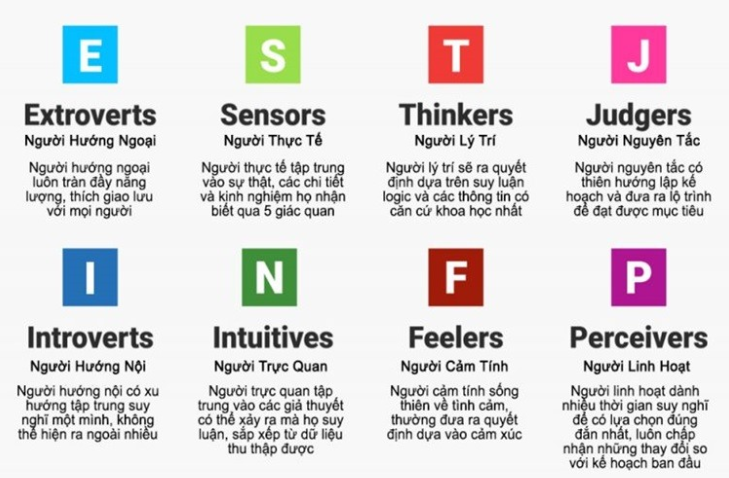
\includegraphics[width=0.8\linewidth, height=0.3\textheight]{images/MBTIper.png}
    \vspace{0.6cm}
    \caption{Ý nghĩa những chữ cái trong tính cách MBTI}
\end{figure}

Các bước đánh giá MBTI bao gồm : 
\begin{itemize}
    \item \textbf{Bước 1:} Trả lời Bộ Câu Hỏi MBTI Đánh giá MBTI bắt đầu với việc trả lời một bộ câu hỏi tự đánh giá. Câu hỏi này được thiết kế để đánh giá các xu hướng tâm lý học của một người trong bốn lĩnh vực chính: Hướng ngoại/Hướng nội, Cảm nhận/Trực giác, Tư duy/Cảm xúc, và Phán đoán/Nhận thức.
    \item \textbf{Bước 2}: Xác Định Loại Tính Cách Dựa trên câu trả lời, mỗi người sẽ được phân loại vào một trong 16 loại tính cách MBTI. Mỗi loại tính cách được biểu diễn bằng một mã gồm bốn chữ cái, mỗi chữ cái đại diện cho một trong các cực đối lập trên.
    \item \textbf{Bước 3:} Phân Tích Kết Quả Sau khi xác định được loại tính cách, người tham gia sẽ nhận được một báo cáo chi tiết về loại tính cách của mình. Báo cáo này thường bao gồm thông tin về điểm mạnh, điểm yếu, phong cách làm việc, và khuyến nghị về sự nghiệp.
    \item \textbf{Bước 4:} Sử Dụng Thông Tin Để Phát Triển Cá Nhân Thông tin từ báo cáo MBTI có thể được sử dụng để hỗ trợ phát triển cá nhân, quản lý sự nghiệp, và cải thiện mối quan hệ cá nhân và nghề nghiệp.
\end{itemize}

MBTI được sử dụng trong nhiều lĩnh vực khác nhau, từ phát triển cá nhân đến quản lý nhân sự trong doanh nghiệp. Nó giúp mọi người hiểu rõ hơn về điểm mạnh và điểm yếu của bản thân, cũng như cách họ có thể tương tác hiệu quả hơn với người khác có tính cách khác biệt. Trong môi trường làm việc, MBTI có thể giúp quản lý xác định đúng người cho đúng vị trí, cải thiện giao tiếp và xây dựng đội nhóm mạnh mẽ hơn.

\subsection{Career Clusters Interest Survey}\label{2.1.3}
\textbf{Career Clusters Interest Survey} là một công cụ hướng nghiệp được phát triển bởi Oklahoma Department of Career and Technology Education. Mục đích của bộ công cụ này là giúp học sinh và người lao động xác định sở thích nghề nghiệp và liên kết chúng với các lĩnh vực nghề nghiệp cụ thể. Đây là một phần của hệ thống hướng nghiệp rộng lớn mà cơ quan này cung cấp, nhằm mục đích hỗ trợ cá nhân trong việc lập kế hoạch sự nghiệp và phát triển kỹ năng.

Career Clusters Interest Survey dựa trên mô hình 16 Career Clusters, mỗi cluster đại diện cho một nhóm nghề nghiệp có liên quan đến nhau dựa trên các kỹ năng và kiến thức chung. 

Các cụm bao gồm :
\begin{itemize}
    \item \textit{Nông nghiệp, Thực phẩm và Tài nguyên thiên nhiên:} Ngành này bao gồm các sự nghiệp liên quan đến nông nghiệp, thực phẩm và tài nguyên thiên nhiên, từ quản lý nông trại đến bảo tồn môi trường.
    \item \textit{Kiến trúc và xây dựng:} Bao gồm các nghề nghiệp trong lĩnh vực kiến trúc, thiết kế và xây dựng, từ việc tạo ra các công trình mới đến bảo trì và sửa chữa cơ sở hạ tầng hiện có.
    \item \textit{Nghệ thuật, Công nghệ A/V và Truyền thông:} Tập trung vào các ngành nghề liên quan đến nghệ thuật, công nghệ âm thanh/visual và truyền thông, từ sản xuất phim đến thiết kế đồ họa.
    \item \textit{Kinh doanh, quản lí và quản trị:} Bao gồm các sự nghiệp trong quản trị kinh doanh và hành chính, từ quản lý văn phòng đến phân tích tài chính.
    \item \textit{Giáo dục và đào tạo:} Ngành này tập trung vào sự nghiệp trong giáo dục và đào tạo, từ giáo viên đến nhà phát triển chương trình giáo dục.
    \item \textit{Tài chính:} Bao gồm các nghề nghiệp liên quan đến tài chính, từ kế toán đến tư vấn đầu tư.
    \item \textit{Chính phủ và hành chính công:} Tập trung vào các sự nghiệp trong chính phủ và quản trị công, từ làm việc trong cơ quan chính phủ đến phục vụ công tác xã hội.
    \item \textit{Y tế:} Bao gồm các nghề nghiệp trong lĩnh vực y tế, từ y tá và bác sĩ đến nghiên cứu khoa học sức khỏe.
    \item \textit{Khách sạn – Nhà hàng – Du lịch}: Tập trung vào các sự nghiệp trong ngành khách sạn và du lịch, từ quản lý khách sạn đến tổ chức tour du lịch.
    \item \textit{Dịch vụ con người:} Bao gồm các nghề nghiệp liên quan đến dịch vụ con người, từ làm việc xã hội đến tư vấn cá nhân.
    \item \textit{Công nghệ thông tin:} Tập trung vào các sự nghiệp trong công nghệ thông tin, từ phát triển phần mềm đến quản trị mạng.
    \item \textit{Luật, An toàn công cộng, Sửa chữa và bảo mật:} Bao gồm các nghề nghiệp liên quan đến luật, an ninh công cộng và sửa chữa, từ luật sư đến cảnh sát.
    \item \textit{Sản xuất:} Tập trung vào các sự nghiệp trong sản xuất, từ quản lý nhà máy đến kỹ thuật sản xuất.
    \item \textit{Marketing:} Bao gồm các nghề nghiệp trong tiếp thị, từ nghiên cứu thị trường đến quảng cáo.
    \item \textit{Khoa học, công nghệ, kỹ thuật và toán học (STEM):} Tập trung vào các sự nghiệp trong khoa học, công nghệ, kỹ thuật và toán học, từ nghiên cứu khoa học đến phát triển công nghệ.
    \item \textit{Phân phối hậu cần:} Bao gồm các nghề nghiệp liên quan đến vận tải, phân phối và logistics, từ lái xe tải đến quản lý chuỗi cung ứng
\end{itemize}
Người dùng sẽ trả lời một loạt câu hỏi được thiết kế để đánh giá sở thích cá nhân và xu hướng nghề nghiệp. Câu hỏi bao gồm các hoạt động, phẩm chất cá nhân và môn học yêu thích. Dựa trên số lượng câu trả lời chọn lựa, người dùng có thể xác định được Career Clusters hàng đầu phù hợp với sở thích và khả năng của họ. 

Bộ công cụ này cung cấp một cách tiếp cận hệ thống để học sinh và người lao động khám phá sự phù hợp nghề nghiệp. Nó giúp người dùng hiểu rõ hơn về bản thân và định hình sự nghiệp dựa trên sở thích và khả năng thực tế. Đồng thời, nó cũng là một nguồn tài liệu tham khảo quý giá cho các nhà giáo dục và cố vấn hướng nghiệp trong việc hỗ trợ học sinh của họ.
\begin{figure}[H]
    \centering
    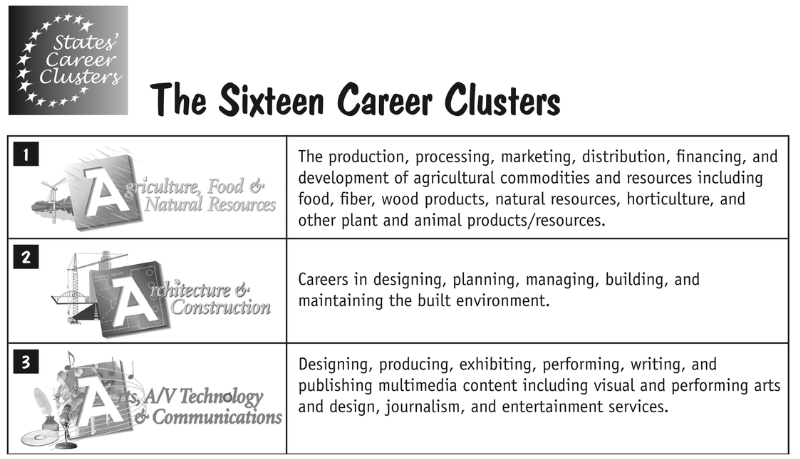
\includegraphics[width=0.5\linewidth]{images/CC.png}
    \vspace{0.6cm}
    \caption{Các cụm nghề nghiệp chính}
\end{figure}
Career Clusters Interest Survey được sử dụng rộng rãi trong các trường học và tổ chức hướng nghiệp ở Oklahoma. Nó giúp học sinh lập kế hoạch học tập và phát triển nghề nghiệp, từ việc chọn lớp học phù hợp đến việc xác định các cơ hội đào tạo và việc làm sau khi tốt nghiệp. Không chỉ hỗ trợ cá nhân trong việc lập kế hoạch sự nghiệp mà Career Clusters Interest Survey còn được  góp phần vào việc phát triển nguồn nhân lực chất lượng cao cho bang Oklahoma và trên toàn nước Mỹ. Hiện nay Career Clusters Interest Survey được rất nhiều nơi, tổ chức về giáo dục trên thế giới sử dụng và đạt hiệu quả vô cùng đáng kể. 

\subsection{MCDM - Multiple-criteria decision-making }
\textbf{Phân tích Quyết định Đa Tiêu Chí (MCDM)} là một lĩnh vực quan trọng trong nghiên cứu hoạt động, giúp ra quyết định khi có nhiều tiêu chí xung đột cần được xem xét. Nguồn gốc của Phân tích Quyết định Đa Tiêu Chí (MCDM) có thể truy nguyên từ những năm 1960, khi các nhà nghiên cứu bắt đầu nhận ra rằng các quyết định trong thực tế thường phải đối mặt với nhiều tiêu chí xung đột và không thể giải quyết chỉ bằng một tiêu chí đơn lẻ. MCDM là một lĩnh vực nghiên cứu liên ngành, kết hợp giữa toán học, kinh tế học, và khoa học quản lý, để giải quyết các vấn đề ra quyết định phức tạp. \\
Stanley Zionts đã giúp phổ biến thuật ngữ này với bài báo năm 1979 mang tên \textit{"MCDM – If not a Roman Numeral, then What?"}, hướng tới đối tượng là các nhà khởi nghiệp. MCDM liên quan đến việc cấu trúc và giải quyết các vấn đề về quyết định và lập kế hoạch liên quan đến nhiều tiêu chí. Mục đích là hỗ trợ những người ra quyết định phải đối mặt với những vấn đề như vậy. Thông thường, không tồn tại một giải pháp tối ưu duy nhất cho các vấn đề như vậy và cần phải sử dụng sở thích của người ra quyết định để phân biệt giữa các giải pháp. "Giải quyết" có thể được hiểu theo những cách khác nhau. Nó có thể tương ứng với việc chọn lựa "phương án tốt nhất" từ một tập hợp các phương án khả dụng (trong đó "tốt nhất" có thể được hiểu là "phương án được ưu tiên nhất" của người ra quyết định). \\
Một cách hiểu khác về "giải quyết" có thể là chọn một tập hợp nhỏ các phương án tốt, hoặc nhóm các phương án thành các tập hợp ưu tiên khác nhau. Cách hiểu đơn giản đó là tìm tất cả các phương án "hiệu quả" hoặc "không bị thống trị" . Độ khó của vấn đề bắt nguồn từ việc có nhiều hơn một tiêu chí. Không còn một giải pháp tối ưu duy nhất cho vấn đề MCDM mà có thể đạt được mà không cần kết hợp thông tin về sở thích. Khái niệm về giải pháp tối ưu thường được thay thế bằng tập các giải pháp không bị thống trị. Một giải pháp được gọi là không bị thống trị nếu không thể cải thiện nó theo bất kỳ tiêu chí nào mà không phải đánh đổi ở một tiêu chí khác. Do đó, người ra quyết định nên chọn một giải pháp từ tập hợp các giải pháp không bị thống trị. Ngược lại, họ có thể làm tốt hơn về một số hoặc tất cả các tiêu chí và không tệ hơn ở bất kỳ tiêu chí nào trong số đó. Tuy nhiên, nhìn chung, tập hợp các giải pháp không bị thống trị quá lớn để trình bày cho người ra quyết định lựa chọn cuối cùng. Do đó, chúng ta cần các công cụ giúp người ra quyết định tập trung vào các giải pháp (hoặc phương án) được ưu tiên. Thông thường, người ta phải "đánh đổi" giữa các tiêu chí này với các tiêu chí khác. Theo góc nhìn từ lịch sử trong cuốn Köksalan, M., Wallenius, J., and Zionts, S. (2011). \textit{Multiple Criteria Decision Making: From Early History to the 21st Century.} MCDM có thể áp dụng trong nhiều lĩnh vực khác nhau như Mathematics, Decision analysis, Economics, Computer technology, Software engineering, Information systems. 

\begin{figure}[H]
    \centering
    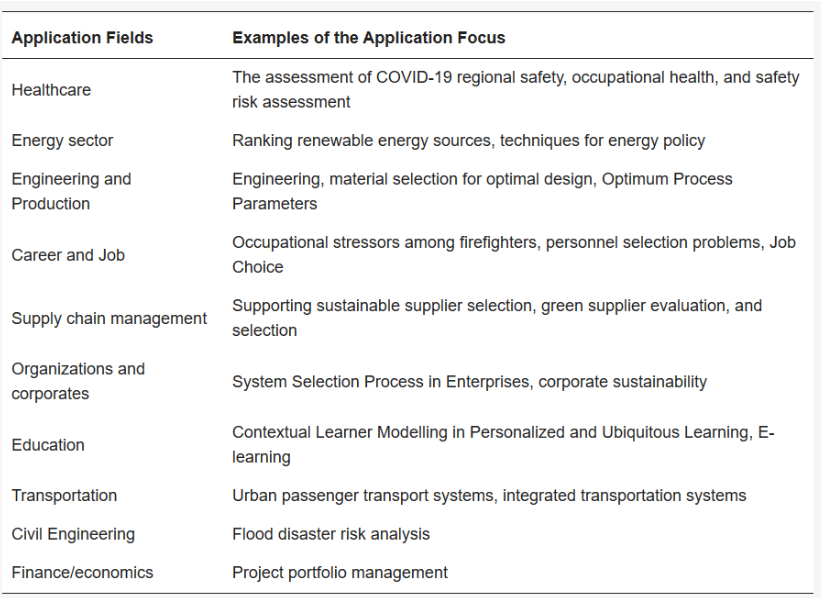
\includegraphics[width=0.8\linewidth, height=0.3\textheight]{images/MCDM.png}
    \vspace{0.6cm}
    \caption{Ứng dụng phương pháp MCDM trong các lĩnh vực}
\end{figure}


Các nhà nghiên cứu như Keeney và Raiffa là những người tiên phong trong việc phát triển khái niệm và phương pháp MCDM. Họ đã đặt nền móng cho việc sử dụng các mô hình toán học để đánh giá và so sánh các lựa chọn dựa trên nhiều tiêu chí khác nhau. Các phương pháp MCDM ban đầu bao gồm Phân Tích Hệ Thống Cấp Bậc (AHP) và Phương pháp TOPSIS, được phát triển để giúp người ra quyết định tìm ra lựa chọn tối ưu nhất khi đối mặt với nhiều tiêu chí đánh giá. \cite{thutucphapluat}

Trong vài thập kỷ gần đây, nhiều phương pháp ra quyết định đa tiêu chí (MCDM) đã được các tác giả khác nhau phát triển hoặc cải tiến. Sự khác biệt chính giữa các phương pháp này liên quan đến mức độ phức tạp của thuật toán, phương pháp trọng số cho các tiêu chí, cách thể hiện tiêu chí đánh giá theo sở thích, khả năng xử lý dữ liệu không chắc chắn và cuối cùng là kiểu tổng hợp dữ liệu 

Mỗi loại giải thuật MCDM khác nhau đều có những ưu nhược điểm riêng biệt cần được giải thích cụ thể dựa trên từng phương pháp. Ví dụ, Quy trình phân cấp Analytic (AHP) dễ sử dụng nhưng gặp vấn đề do sự phụ thuộc lẫn nhau giữa các tiêu chí và lựa chọn. Mặt khác, Lý thuyết tập Fuzzy (FST) có thể sử dụng đầu vào không chính xác; tuy nhiên, phương pháp này lại không dễ phát triển. Nhìn chung, tất cả các phương pháp MCDM đều có ưu điểm là xem xét tác động không cân đối và mâu thuẫn của các quyết định. Mặt hạn chế là các giải pháp do các phương pháp này tạo ra thường là sự thỏa hiệp giữa nhiều mục tiêu và do bản chất của vấn đề nên không đạt được điểm tối ưu. 

MCDM bao gồm các yếu tố và khái niệm khác nhau tùy thuộc vào bản chất của vấn đề ra quyết định. Các yếu tố chính thường được đề cập tới bao gồm:
\begin{itemize}
    \item Các lựa chọn (Alternatives): Là "những cách hành động khả thi khác nhau".
    \item Thuộc tính (Attribute): "đặc điểm có thể đo lường được của một lựa chọn".
    \item Tổng hợp (Aggregation) : "xem xét hiệu quả của một lựa chọn trên các tiêu chí cụ thể để đưa ra quyết định về lựa chọn đó".
    \item Biến quyết định (Decision variables): “các thành phần của vector lựa chọn".
\item Không gian quyết định(Decision space): "Các lựa chọn khả thi".
\item Đo lường (Measures) : "các yếu tố được sử dụng để lượng hóa một lựa chọn theo thuộc tính của nó bằng cách gán cho thuộc tính các số hoặc ký hiệu".
\item Tiêu chí (Criteria): "công cụ để đánh giá và so sánh các lựa chọn theo quan điểm về hậu quả của việc lựa chọn chúng".
\item Sở thích (Preferences): Được định nghĩa là "cách thức một lựa chọn đáp ứng nhu cầu của người ra quyết định đối với một thuộc tính nhất định".
\item Quyết định (Decisions) :Có thể khác nhau dựa trên loại vấn đề, bao gồm các vấn đề lựa chọn, xếp hạng và phân loại

\end{itemize}


Có những cách hiểu khác nhau về việc giải quyết vấn đề MCDM. Quá trình này có thể được coi là chọn ra lựa chọn tốt nhất (ưu tiên nhất) từ một tập hợp các lựa chọn. Nó cũng có thể được giải thích như việc nhóm các lựa chọn (thành nhiều tập ưu tiên) và sau đó chọn một tập nhỏ từ chúng. Hơn nữa, các vấn đề này nhằm mục đích xác định các lựa chọn không bị chi phối hoặc hiệu quả. Không có cách nào để chuyển từ một giải pháp không bị chi phối sang một giải pháp khác mà không hy sinh ít nhất một trong các tiêu chí, điều này có thể giúp người ra quyết định lựa chọn một tập hợp giải pháp từ tập các giải pháp không bị chi phối. Để giải quyết vấn đề MCDM, ta đi theo các bước tuần tự sau : 
\begin{figure}[H]
    \centering
    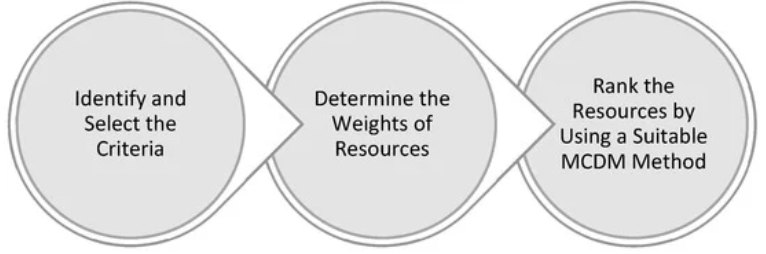
\includegraphics[width=0.8\linewidth, height=0.25\textheight]{images/MCDMstep.png}
    \caption{Các bước giải quyết vấn đề MCDM}
\end{figure}
Hoặc cụ thể hơn là \cite{davood}:
\begin{figure}[H]
    \centering
    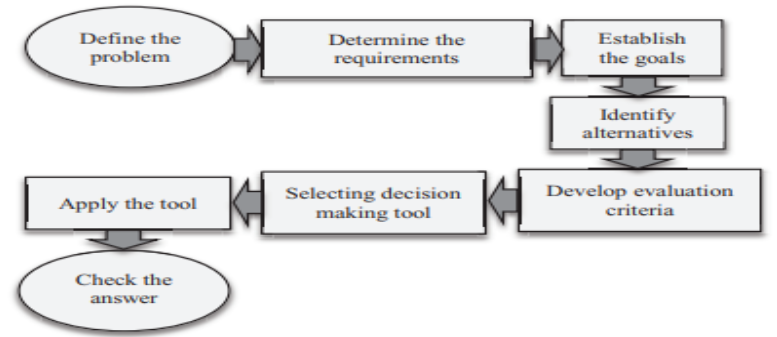
\includegraphics[width=0.8\linewidth, height=0.25\textheight]{images/MCDMdiagram.png}
    \caption{Quy trình ra quyết định chung}
    \vspace{0.6cm
    }
\end{figure}

Có nhiều phương pháp MCDM với các đặc điểm khác nhau có thể liên quan đến nhiều khía cạnh từ chất lượng của câu trả lời đến loại vấn đề mà các phương pháp này giải quyết. Do đó, để có được sự hiểu biết tốt hơn về các phương pháp luận MCDM giúp chọn phương pháp phù hợp cho các vấn đề đối mặt, việc xác định phân loại các vấn đề MCDM là cần thiết. Các kiểu loại và nhóm phụ khác nhau xem xét các khía cạnh khác nhau của vấn đề được nhận diện trong nhiều nghiên cứu. 

\begin{figure}[H]
    \centering
    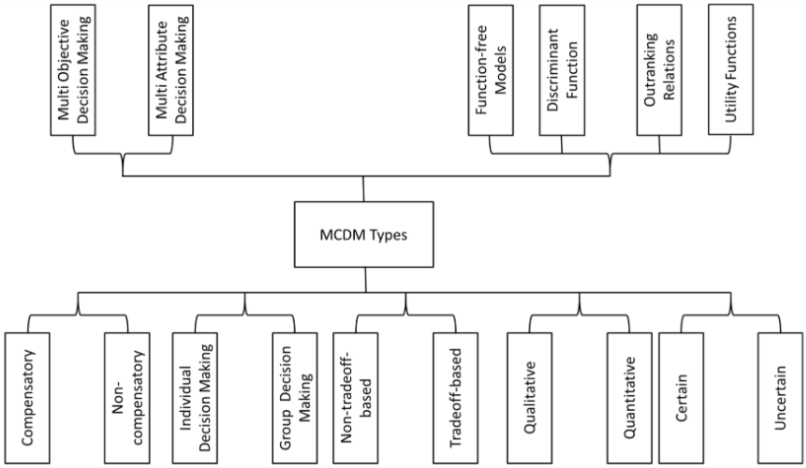
\includegraphics[width=0.8\linewidth, height=0.35\textheight]{images/MCDMtype.png}
    \vspace{0.6cm}
    \caption{Phân loại các phương pháp luận MCDM}
\end{figure}

Như đã giới thiệu về một vài giải thuật MCDM, hiện nay, một số giải thuật MCDM phổ biến và được sử dụng rộng rãi trên thế giới bao gồm \cite{sciencedirect1}: 

\begin{itemize}
    \item \textit{AHP (Analytic Hierarchy Process):} AHP là một phương pháp phổ biến được sử dụng để giải quyết các vấn đề quyết định phức tạp. Phương pháp này sử dụng một cấu trúc phân cấp để đánh giá các tiêu chí và lựa chọn, giúp người ra quyết định có thể so sánh các yếu tố một cách hệ thống.
    \item \textit{TOPSIS (Technique for Order Preference by Similarity to Ideal Solution)}: TOPSIS chọn lựa phương án có khoảng cách Euclidean ngắn nhất từ giải pháp lý tưởng và xa nhất từ giải pháp lý tưởng tiêu cực. Phương pháp này thường được sử dụng trong các tình huống mua sắm hoặc lựa chọn sản phẩm dựa trên nhiều tiêu chí khác nhau1.
    \item \textit{VIKOR (VIseKriterijumska Optimizacija I Kompromisno Resenje)}: VIKOR tập trung vào việc tìm ra giải pháp tối ưu khi có sự đối lập giữa các tiêu chí. Phương pháp này giúp xác định giải pháp cân bằng giữa các tiêu chí khác nhau.
    \item \textit{ELECTRE (Elimination and Choice Expressing Reality)}: ELECTRE sử dụng các phương pháp so sánh cặp để xếp hạng các lựa chọn. Nó xem xét sự không tương thích giữa các tiêu chí và loại bỏ các lựa chọn không phù hợp.

    \item \textit{PROMETHEE (Preference Ranking Organization METHod for Enrichment Evaluations)}: PROMETHEE là một phương pháp khác sử dụng so sánh cặp và được ưa chuộng trong các quyết định liên quan đến môi trường và quản lý tài nguyên.

    \item \textit{MOORA (Multi-Objective Optimization by Ratio Analysis)}: MOORA là một phương pháp tối ưu hóa đa mục tiêu sử dụng phân tích tỷ lệ để đánh giá các lựa chọn dựa trên nhiều tiêu chí.

\item \textit{COPRAS (COmplex PRoportional ASsessment)}: COPRAS xem xét sự phức tạp của các tiêu chí và đánh giá chúng một cách tỷ lệ để tìm ra lựa chọn tốt nhất.

\item \textit{SAW (Simple Additive Weighting)}: SAW là một phương pháp đơn giản nhưng hiệu quả, nó cộng dồn các giá trị đã được chuẩn hóa của các tiêu chí sau khi đã nhân với trọng số tương ứng.

\item \textit{MAVT (Multi-Attribute Value Theory)}: MAVT sử dụng lý thuyết giá trị để đánh giá các lựa chọn dựa trên nhiều tiêu chí. Phương pháp này thường được áp dụng trong các quyết định chính sách và quản lý.

\item \textit{MACBETH (Measuring Attractiveness by a Categorical Based Evaluation Technique)}: MACBETH là một phương pháp đánh giá dựa trên các hạng mục và được sử dụng để đo lường sức hấp dẫn của các lựa chọn.

\end{itemize}

Ngoài ra còn có những giải thuật khác được liệt kê trong hình dưới đây : 

\begin{figure}[H]
    \centering
    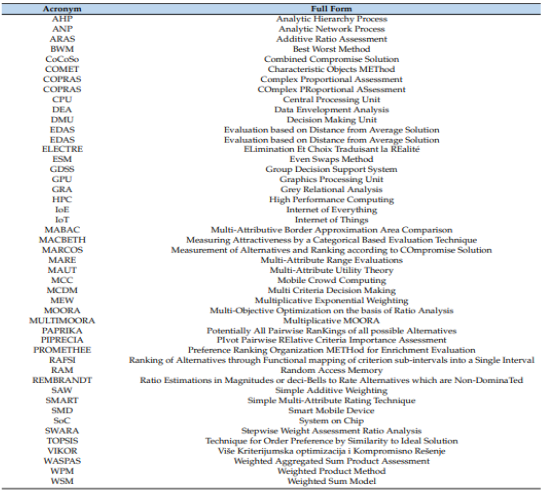
\includegraphics[width=0.8\linewidth,height=0.3\textheight]{images/MCDMalgorithm.png}
    \vspace{0.6cm}
    \caption{Tổng hợp giải thuật MCDM \cite{pijush}}
\end{figure}

Các giải thuật MCDM này đều có những ưu điểm và hạn chế riêng, tùy thuộc vào bối cảnh và yêu cầu cụ thể của từng vấn đề quyết định mà người ra quyết định sẽ lựa chọn phương pháp phù hợp nhất. Việc áp dụng các giải thuật MCDM giúp tối ưu hóa quá trình ra quyết định, đặc biệt trong các tình huống đòi hỏi sự cân nhắc giữa nhiều tiêu chí khác nhau. 

Để có thể thấy được tầm ảnh hưởng của MCDM, chúng ta cùng xem xét biểu đồ sau: 
\begin{figure}[H]
    \centering
    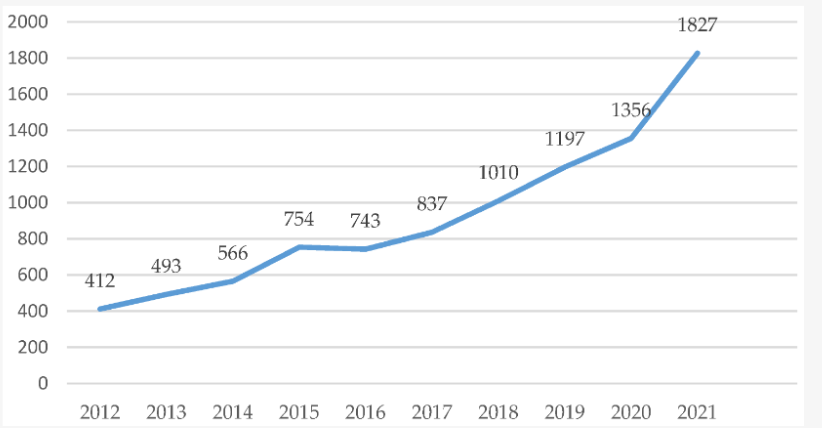
\includegraphics[width=0.5\linewidth]{images/MCDMgraph.png}
    \vspace{0.6cm}
    \caption{Sự gia tăng việc sử dụng phương pháp MCDM trong nghiên cứu}
\end{figure}

Hình ảnh cho thấy rõ sự gia tăng kết quả nghiên cứu trong những năm gần đây, chứng tỏ sự phổ biến của các phương pháp MCDM trong các nghiên cứu gần đây. Giải thuật thuật MCDM có liên quan trực tiếp đến các giải pháp cho các vấn đề về tính bền vững. Điều này nhấn mạnh tầm quan trọng của các kỹ thuật MCDM và sự phát triển nhanh chóng của chúng. 

Mặt khác, như đã đề cập trong các phần trước, các phương pháp MCDM được sử dụng trong nhiều lĩnh vực, từ năng lượng đến kinh doanh. Để minh họa, hình ảnh dưới đây thể hiện số lượng bài nghiên cứu theo lĩnh vực (xét trường hợp một số bài nghiên cứu có thể thuộc nhiều lĩnh vực). Kết quả cho thấy các phương pháp MCDM được sử dụng trong rất nhiều lĩnh vực nghiên cứu, chẳng hạn như toán học, năng lượng, khoa học máy tính, v.v.
\begin{figure}[H]
    \centering
    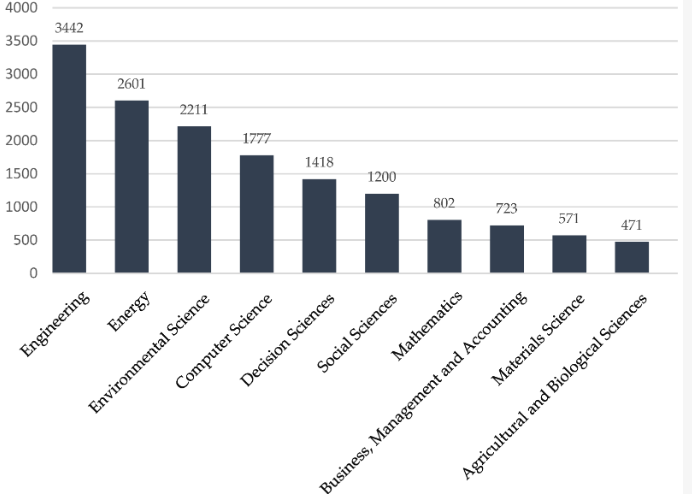
\includegraphics[width=0.65\linewidth]{images/MCDMarea.png}
    \vspace{0.6cm}
    \caption{Các lĩnh vực nghiên cứu bằng phương pháp MCDM}
\end{figure}

MCDM là một công cụ quý giá trong việc ra quyết định khi cần xem xét nhiều tiêu chí thường xung đột với nhau. Nó cung cấp một cách tiếp cận có cấu trúc có thể dẫn đến quyết định thông tin đầy đủ và tốt hơn. Mặc dù có những thách thức liên quan đến việc sử dụng nó, nhưng lợi ích của việc áp dụng các kỹ thuật MCDM trong các tình huống ra quyết định phức tạp là đáng kể. Theo những nghiên cứu gần đây, MCDM sẽ còn phát triển và trở thành một trong những công cụ mạnh mẽ nhất để giải quyết những bài toán cần đưa ra lựa chọn hay quyết định.

\subsection{VIKOR}

Như đã giới thiệu ở phần trên về MCDM, trong số các giải thuật MCDM trong đồ án này sẽ tập trung phát triển vào giải thuật \textbf{VIKOR} - Vlsekriterijumska Optimizacija I Kompromisno Resenje - theo tiếng Serbia có nghĩa là tối ưu hóa đa tiêu chí và giải pháp thỏa hiệp - là một phương pháp ra quyết định đa tiêu chí được phát triển vào năm 1990 bởi Serafim Opricovic để giải quyết các vấn đề quyết định với các tiêu chí xung đột. Phương pháp này xếp hạng các lựa chọn và xác định giải pháp thỏa hiệp gần nhất với "giải pháp lý tưởng".

Sự gia tăng nhanh chóng việc sử dụng VIKOR trong thực tế được minh chứng bởi hơn 200 bài báo khoa học và hội nghị quốc tế. Trong đó đánh giá VIKOR là một giải thuật hiệu quả so sáng với các phương pháp, giải thuật MCDM khác theo (Opricovic, 2011; Kang, 2014). 

Phương pháp VIKOR bao gồm việc tối ưu đa tiêu chí cho các hệ thống phức tạp, tập trung vào việc xếp hạng và lựa chọn từ một tập các phương án thay thế trong số các tiêu chí xung đột. Vai trò của nó là tìm ra chỉ số xếp hạng đa tiêu chí dựa trên thước đo cụ thể về độ gần với giải pháp lý tưởng VIKOR giúp giải quyết các vấn đề ra quyết định đa tiêu chí (MCDM) nhờ hai ưu điểm: cung cấp tập tối đa các khả năng và giảm thiểu tối đa tính “hối hận” khi đưa ra quyết định được lụa chọn. Xếp hạng các phương án của VIKOR có bốn bước, 
Trong đó n và m lần lượt là số tiêu chí và phương án. Quy trình toán học được trình bày trong Hình sau \cite{morteza}. 

\begin{figure}[H]
    \centering
    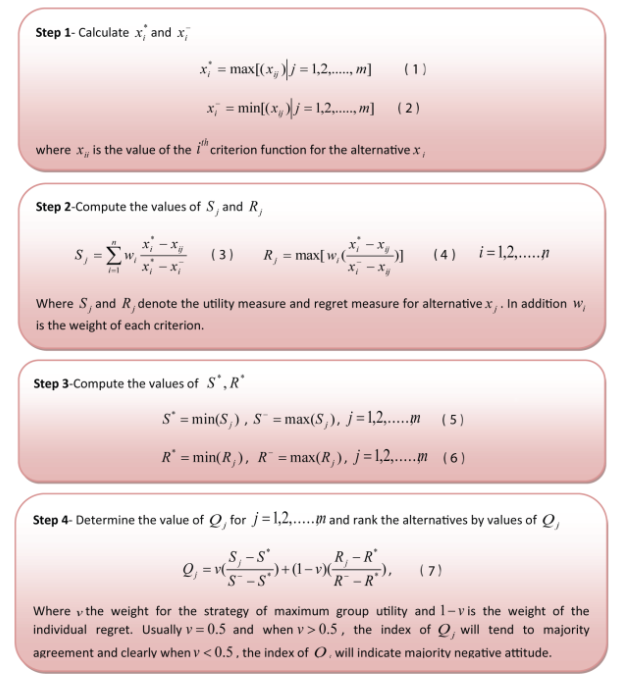
\includegraphics[width=0.8\linewidth, height=0.3\textheight]{images/VIKOR.png}
    \vspace{0.6cm}
    \caption{Các bước trong quy trình }
\end{figure}

\begin{itemize}
    \item Bước 1 và 2 tìm ra đo lường tiêu chí và đo lường “hối tiếc” cho các phương án đối với mỗi tiêu chí. 
    \item Sau đó, bước 3 tính toán số lượng tối thiểu và tối đa của kết quả của bước 2. 
    \item Bước 4: Tính toán $Q_j$ như sự đồng thuận của đa số trong ưu tiên các phương án.
\end{itemize}

Từ cách thức thực hiện trên, ta có thể thấy rằng Vikor có một số điểm mạnh và điểm yếu so với các giải thuật MCDM khác. 
\begin{itemize}
    \item Ưu điểm:
        \begin{itemize}
            \item \textit{Dễ hiểu và sử dụng}: 
            Vikor sử dụng một phương pháp tiếp cận thỏa hiệp đơn giản để xác định giải pháp tốt nhất, dễ hiểu và áp dụng cho người dùng không có chuyên môn về MCDM. Cân nhắc đồng thời cả độ chênh lệch so với giá trị lý tưởng và độ hối tiếc: Vikor sử dụng hai chỉ số, $S$ và $R$, để đánh giá các giải pháp dựa trên cả độ chênh lệch so với giá trị lý tưởng và mức độ hối tiếc nếu chọn giải pháp đó. Điều này giúp đảm bảo rằng giải pháp được chọn không chỉ là giải pháp tốt nhất về mặt lý thuyết mà còn là giải pháp ít gây hối tiếc nhất cho người quyết định. 
            \item \textit{Có thể xử lý các tiêu chí định lượng và định tính: }
Vikor có thể xử lý cả hai loại tiêu chí, giúp nó linh hoạt hơn so với các giải thuật chỉ có thể xử lý một loại tiêu chí. Khả năng điều chỉnh: Vikor cho phép người dùng điều chỉnh các tham số để phù hợp với nhu cầu cụ thể của họ. Ví dụ, người dùng có thể điều chỉnh trọng số của hai chỉ số $S$ và $R$ để ưu tiên một trong hai khía cạnh hơn. 

        \end{itemize}
    \item Nhược điểm:
        \begin{itemize}
            \item \textit{Nhạy cảm với sự thay đổi trong giá trị trọng số: }
Vikor có thể nhạy cảm với sự thay đổi trong giá trị trọng số của các tiêu chí. Do đó, điều quan trọng là phải chọn giá trị trọng số cẩn thận để đảm bảo rằng kết quả phản ánh đúng nhu cầu của người quyết định. Không có quy trình rõ ràng để xác định giá trị trọng số: Vikor không cung cấp một quy trình rõ ràng để xác định giá trị trọng số của các tiêu chí. Điều này có thể dẫn đến kết quả khác nhau tùy thuộc vào cách người dùng chọn giá trị trọng số
        \end{itemize}
\end{itemize}

So sánh VIKOR với các giải thuật MCDM khác: 
\begin{itemize}
    \item \textit{Đối với TOPSIS:} TOPSIS cũng sử dụng một phương pháp tiếp cận thỏa hiệp để xác định giải pháp tốt nhất. Tuy nhiên, TOPSIS tập trung vào việc chọn giải pháp gần với giải pháp lý tưởng nhất, trong khi Vikor cân nhắc cả độ chênh lệch so với giá trị lý tưởng và độ hối tiếc.
    \item \textit{Đối với AHP:} AHP sử dụng một quy trình phân cấp để so sánh các tiêu chí trực tiếp. Tuy nhiên, AHP có thể phức tạp hơn Vikor để thực hiện và nhạy cảm với sự không nhất quán trong đánh giá của người quyết định.
    \item \textit{Đối với ELECTRE:} ELECTRE sử dụng một quy trình loại trừ để xác định giải pháp tốt nhất. Tuy nhiên, ELECTRE có thể phức tạp hơn Vikor để thực hiện và nhạy cảm với sự lựa chọn của các tham số.
\end{itemize}

 Trong nghiên cứu của  Morteza Yazdani và Felipe Reis Gramel có 198 bài nghiên cứu khoa học về VIKOR được tìm kiếm và sắp xếp trong khoảng thời gian từ 2002-2014 \cite{morteza}. 
 \begin{figure}[h]
     \centering
     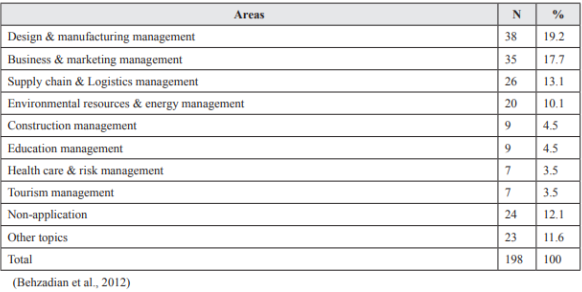
\includegraphics[width=0.8\linewidth,height=0.35\textheight]{images/VIKORtable.png}
 \end{figure}
Cho ta thấy rằng không chỉ có MCDM như đã nói ở phần trên được áp dụng rộng rãi trong nhiều lĩnh vực mà ngay cả VIKOR cũng thế, nó được áp dụng trong nhiều ngành nghề, lĩnh vực, mục đích khác nhau và mang lại hiệu quả đáng kinh ngạc. Bản thân con người khi đưa ra quyết định luôn cân nhắc dựa trên nhiều yếu tố khác nhau, do đó 1 giải pháp tạo ra sự cân nhắc giữa các tiêu chí như VIKOR thực sự rất hiệu quả trong cuộc sống thực tế và điều nó được áp dụng rộng rãi trở nên thành một điều hiển nhiên có thể nhận thấy được.
Phương pháp VIKOR là một công cụ hữu ích và mạnh mẽ trong việc giải quyết các vấn đề quyết định đa tiêu chí trong nhiều lĩnh vực khác nhau. Điều này đặc biệt quan trọng trong thế giới hiện đại nơi mà sự phức tạp và sự đa dạng ngày càng tăng lên trong các quyết định chiến lược và hoạt động hàng ngày.

\subsection{Weighted-sum}
Phương pháp \textbf{Weighted Sum }(Tổng trọng số) là một trong những phương pháp MCDM (Quyết định đa tiêu chí) phổ biến và đơn giản nhất. Phương pháp này sử dụng một tập hợp các trọng số để phản ánh tầm quan trọng của từng tiêu chí và sau đó tổng hợp giá trị của tất cả các tiêu chí để xác định giải pháp tốt nhất.
Cách thức thực hiện:
\begin{itemize}
    \item \textit{Bước 1:} Xác định các tiêu chí:
    Đầu tiên, Cần xác định danh sách các tiêu chí cần đánh giá. Các tiêu chí này thường phản ánh các khía cạnh quan trọng của bài toán. Ví dụ: hiệu suất, chi phí, độ ưu tiên, rủi ro, v.v.
Các tiêu chí có thể được lựa chọn dựa trên kiến thức chuyên môn, ý kiến của người ra quyết định, hoặc thông qua phỏng vấn với các chuyên gia
    \item \textit{Bước 2:} Xác định trọng số cho các tiêu chí:
    Mỗi tiêu chí được gán một trọng số tương ứng, thể hiện mức độ quan trọng của nó trong quyết định.
Trọng số này có thể được xác định dựa trên ý kiến của người ra quyết định hoặc thông qua phương pháp tính toán. Cách thông thường là thảo luận với các chuyên gia hoặc sử dụng phương pháp phân tích so sánh đôi.
    \item \textit{Bước 3:} Đánh giá hiệu suất của các phương án:
    Đối với mỗi phương án, chúng ta đánh giá hiệu suất của nó trên từng tiêu chí.
Điều này có thể dựa trên dữ liệu thực tế (ví dụ: số liệu kỹ thuật, số liệu tài chính) hoặc thông qua đánh giá chủ quan (ví dụ: đánh giá từ người ra quyết định hoặc chuyên gia).
    \item \textit{Bước 4:} Tính toán tổng trọng số:
    Tổng trọng số của mỗi phương án được tính bằng cách nhân hiệu suất của phương án với trọng số tương ứng của từng tiêu chí và tổng hợp chúng lại.
\end{itemize}
Kết quả cuối cùng là một điểm tổng hợp cho mỗi phương án, giúp người ra quyết định so sánh và lựa chọn phương án tốt nhất. Ví dụ, khi chọn ứng viên cho một vị trí công việc, chúng ta có thể đánh giá từng ứng viên dựa trên các tiêu chí như kinh nghiệm, kỹ năng, học vấn và đánh giá trọng số cho mỗi tiêu chí. Sau đó, tổng hợp điểm của từng ứng viên để đưa ra quyết định cuối cùng.\\
Phương pháp weighted-sum là một phương pháp đơn giản và dễ dàng hiện thực, có thể linh hoạt đối với bất cứ đối tượng, tiêu chí nào. Tuy vậy kết quả của phương pháp Weighted Sum có thể nhạy cảm với sự thay đổi trong trọng số của các tiêu chí. Do đó, điều quan trọng là phải chọn trọng số cẩn thận hơn nữa, phương pháp Weighted Sum có thể không phù hợp với các tiêu chí không tương thích, chẳng hạn như chi phí và chất lượng và có thể không phản ánh đầy đủ sự đánh đổi giữa các tiêu chí. cũng như là chưa chắc chắn sự tuyến tính giữa các tiêu chí, tuy vậy ngày nay weighted-sum vẫn được ứng dụng cho những hệ thống đơn giản và là ví dụ tiêu biểu để hiểu và vận dụng mcdm một cách linh hoạt hơn, hơn nữa trong những từng huống cụ thể rõ ràng, weighted-sum có thể phát huy tối đa sự linh động và hiệu quá, đem đến những kết quả hợp lí cho người dùng

\subsection{Python và các thư viện liên quan}
\textbf{Python} là một ngôn ngữ lập trình bậc cao, đa năng, được sử dụng rộng rãi trong nhiều lĩnh vực khác nhau như phát triển web, khoa học dữ liệu, trí tuệ nhân tạo, tự động hóa, v.v. Nó được đánh giá cao bởi tính dễ học, dễ đọc, dễ sử dụng và miễn phí.
\begin{itemize}
    \item Lịch sử ra đời:
    Python được tạo ra bởi Guido van Rossum vào cuối những năm 1980 tại Viện Nghiên cứu Quốc gia về Toán học và Khoa học Máy tính ở Hà Lan. Mục tiêu của ông là tạo ra một ngôn ngữ lập trình đơn giản, dễ học và dễ sử dụng, đồng thời mạnh mẽ và linh hoạt.
    \item Đặc điểm nổi bật:
        \begin{itemize}
            \item Dễ học: Python có cú pháp đơn giản, rõ ràng, gần giống với tiếng Anh tự nhiên, giúp người mới bắt đầu dễ dàng tiếp cận và học ngôn ngữ.
            \item Dễ đọc: Mã Python được viết với số lượng ký tự ít hơn so với các ngôn ngữ khác, đồng thời sử dụng thụt lề để phân chia khối mã, giúp cho mã dễ đọc và dễ hiểu hơn.
            \item Dễ sử dụng: Python cung cấp nhiều thư viện và bộ công cụ tích hợp sẵn cho nhiều tác vụ khác nhau, giúp người lập trình tiết kiệm thời gian và công sức.
            \item Miễn phí: Python là ngôn ngữ mã nguồn mở, được phát hành miễn phí cho mọi người sử dụng và sửa đổi.
            \item Mạnh mẽ và linh hoạt: Python có thể được sử dụng để giải quyết nhiều loại vấn đề khác nhau, từ đơn giản đến phức tạp. Nó hỗ trợ nhiều mô hình lập trình khác nhau như lập trình hướng đối tượng, lập trình chức năng, v.v.
        \end{itemize}
    \item Ứng dụng: 
    Python được sử dụng rộng rãi trong nhiều lĩnh vực khác nhau, bao gồm:
        \begin{itemize}
            \item \textit{Phát triển web}: Python được sử dụng để phát triển các ứng dụng web, trang web, backend API, v.v. với các framework phổ biến như Django, Flask.
            \item \textit{Khoa học dữ liệu:} Python là ngôn ngữ hàng đầu trong lĩnh vực khoa học dữ liệu nhờ khả năng xử lý dữ liệu mạnh mẽ, các thư viện khoa học dữ liệu phong phú như NumPy, Pandas, SciPy, Matplotlib.
            \item \textit{Trí tuệ nhân tạo}: Python được sử dụng để phát triển các mô hình học máy, học sâu, xử lý ngôn ngữ tự nhiên, v.v. với các thư viện như TensorFlow, PyTorch, scikit-learn.
            \item \textit{Tự động hóa:} Python được sử dụng để tự động hóa các tác vụ lặp đi lặp lại, tiết kiệm thời gian và công sức cho người dùng.
            \item \textit{Giáo dục: }Python được sử dụng trong giáo dục để dạy lập trình cho học sinh, sinh viên do tính dễ học và dễ sử dụng.
        \end{itemize}
\end{itemize}
Ngoài ra, Python có một cộng đồng người dùng và nhà phát triển lớn và tích cực trên toàn thế giới. Cộng đồng này luôn hỗ trợ lẫn nhau, chia sẻ kiến thức, kinh nghiệm và phát triển các thư viện, công cụ mới cho ngôn ngữ. Hơn nữa, hiện nay trên indeed có khoảng 27,000 việc làm liên quan tới python, trên toàn cầu, có hơn 8,2 triệu lập trình viên sử dụng Python, vượt qua số lượng người sử dụng Java (khoảng 7,6 triệu) \cite{zdnet} , với mức lương trung bình tại mỹ là khoảng hơn 100,000 đô la mỹ một năm cho thấy tiềm năng phát triển vô cùng to lớn của python .\\
Trong đồ án này, sử dụng thư viện \textbf{Flask} của Python để xây dựng các API(Application Programming Interface) cần thiết cho hệ thống. Flask là một web framework (khung ứng dụng web) nhẹ được viết bằng ngôn ngữ lập trình Python. Nó được thiết kế đơn giản, linh hoạt và dễ sử dụng, giúp các nhà phát triển xây dựng các ứng dụng web nhanh chóng và hiệu quả. Flask không đi kèm với các tính năng tích hợp sẵn như ORM (Object Relational Mapping) hoặc hệ thống templating mặc định, nhưng điều này cho phép người dùng lựa chọn các công cụ phù hợp nhất với nhu cầu.

Ưu điểm của Flask:
\begin{itemize}
    \item \textit{Nhẹ và đơn giản:} Flask là một framework nhỏ gọn và dễ học, lý tưởng cho những người mới bắt đầu phát triển web với Python.
    \item \textit{Linh hoạt:} Flask không áp đặt cấu trúc cụ thể nào lên ứng dụng của bạn, cho phép bạn tự do tùy chỉnh ứng dụng theo nhu cầu của mình.
    \item \textit{Mở rộng:} Flask có thể được mở rộng với nhiều thư viện và extension của bên thứ ba, cung cấp cho bạn nhiều chức năng hơn cho ứng dụng web của mình.
    \item \textit{Dễ sử dụng:} Flask cung cấp một API đơn giản và dễ hiểu, giúp bạn dễ dàng xây dựng các ứng dụng web.
    \item \textit{Hiệu suất cao:} Flask được tối ưu hóa cho hiệu suất cao, giúp ứng dụng web của bạn chạy nhanh và mượt mà.
\end{itemize}

 Với nhiều chức năng như : Routing, Templating, Sessions, Request handling, Error handling,... Flask là một lựa chọn tuyệt vời cho các nhà phát triển Python muốn xây dựng các ứng dụng web nhanh chóng, dễ dàng và hiệu quả. Với sự đơn giản, linh hoạt và hiệu suất cao, Flask đã trở thành một trong những web framework Python phổ biến nhất hiện nay.

Ngoài ra trong đồ án còn sử dụng 1 thư viện chính để xử lý dữ liệu là \textbf{Pandas}. Pandas là một thư viện mã nguồn mở mạnh mẽ và linh hoạt được viết bằng ngôn ngữ lập trình Python, được thiết kế dành cho việc phân tích dữ liệu và xử lý dữ liệu. Nó cung cấp các cấu trúc dữ liệu hiệu quả và các công cụ mạnh mẽ để thao tác, làm sạch, phân tích và trực quan hóa dữ liệu. Pandas được sử dụng rộng rãi trong nhiều lĩnh vực khác nhau, bao gồm khoa học dữ liệu, tài chính, kinh doanh, nghiên cứu khoa học và học thuật.

Ưu điểm của Pandas:
\begin{itemize}
    \item \textit{Dễ sử dụng:} Pandas cung cấp một API đơn giản và dễ hiểu, giúp người dùng dễ dàng học cách sử dụng và thao tác dữ liệu.
    \item \textit{Hiệu quả:} Pandas được tối ưu hóa cho hiệu suất cao, giúp xử lý dữ liệu nhanh chóng và hiệu quả, ngay cả với các tập dữ liệu lớn.
    \item \textit{Linh hoạt:} Pandas hỗ trợ nhiều loại dữ liệu khác nhau, bao gồm bảng tính, chuỗi thời gian, dữ liệu ma trận và dữ liệu phi cấu trúc.
    \item \textit{Mạnh mẽ:} Pandas cung cấp nhiều công cụ mạnh mẽ để thao tác, làm sạch, phân tích và trực quan hóa dữ liệu.
    \item \textit{Phổ biến:} Pandas là một thư viện phổ biến với cộng đồng người dùng lớn và nhiều tài nguyên hỗ trợ sẵn có.
\end{itemize}

Pandas là một thư viện Python thiết yếu cho bất kỳ ai làm việc với dữ liệu. Với sự dễ sử dụng, hiệu quả, tính linh hoạt và sức mạnh của nó, Pandas đã trở thành công cụ được lựa chọn cho việc phân tích dữ liệu và xử lý dữ liệu trong Python.

\subsection{MongoDB}

\textbf{MongoDB} là một hệ quản trị cơ sở dữ liệu NoSQL mã nguồn mở đa nền tảng được viết bằng C++. Nó được thiết kế để lưu trữ, truy vấn và quản lý dữ liệu phi cấu trúc, thường được gọi là dữ liệu dạng tài liệu (document-oriented data). MongoDB lưu trữ dữ liệu dưới dạng các bộ sưu tập (collections) gồm các tài liệu (documents), tương tự như các đối tượng JSON.
\begin{itemize}
    \item Ưu điểm của MongoDB:

        \begin{itemize}
            \item \textit{Dễ sử dụng:} MongoDB cung cấp một API đơn giản và dễ hiểu, giúp người dùng dễ dàng học cách sử dụng và lưu trữ dữ liệu phi cấu trúc.
            \item \textit{Linh hoạt:} MongoDB có thể lưu trữ nhiều loại dữ liệu phi cấu trúc khác nhau, bao gồm JSON, BSON, và CSV.
            \item \textit{Mở rộng:} MongoDB có thể mở rộng theo chiều ngang để xử lý khối lượng dữ liệu lớn và lưu lượng truy cập cao.
            \item \textit{Hiệu suất cao:} MongoDB được tối ưu hóa cho hiệu suất cao, giúp truy cập dữ liệu nhanh chóng và hiệu quả.
            \item \textit{Phổ biến:} MongoDB là một hệ quản trị cơ sở dữ liệu NoSQL phổ biến với cộng đồng người dùng lớn và nhiều tài nguyên hỗ trợ sẵn có.
        \end{itemize}

    \item Các tính năng chính của MongoDB:
        \begin{itemize}
            \item \textit{Dữ liệu phi cấu trúc}: MongoDB lưu trữ dữ liệu dưới dạng các tài liệu phi cấu trúc, cho phép lưu trữ dữ liệu linh hoạt và dễ dàng thay đổi.
            \item \textit{Sơ đồ linh hoạt:} MongoDB không sử dụng sơ đồ cố định cho dữ liệu, cho phép người dùng lưu trữ dữ liệu theo cách phù hợp với nhu cầu của họ.
            \item \textit{Truy vấn mạnh mẽ}: MongoDB cung cấp ngôn ngữ truy vấn mạnh mẽ (MongoDB Query Language - MQL) để truy vấn dữ liệu phi cấu trúc.
            \item \textit{Hỗ trợ nhiều ngôn ngữ:} MongoDB hỗ trợ nhiều ngôn ngữ lập trình khác nhau, bao gồm Python, Java, C++, JavaScript, và hơn thế nữa.
            \item \textit{Phân phối:} MongoDB có thể được triển khai theo cụm (cluster) để tăng khả dụng và hiệu suất.
        \end{itemize}
\end{itemize}

Trong đồ án này sử dụng \textbf{MongoDB Atlas}, phiên bản online server của MongoDB được chính nhà phát triển của MongoDB xây dựng. MongoDB Atlas là một hệ quản trị cơ sở dữ liệu NoSQL mạnh mẽ và linh hoạt lý tưởng cho việc lưu trữ, truy vấn và quản lý dữ liệu phi cấu trúc. Với sự dễ sử dụng, tính linh hoạt, hiệu suất cao và cộng đồng người dùng lớn, MongoDB đã trở thành một lựa chọn phổ biến cho các ứng dụng web hiện đại và các ứng dụng dữ liệu lớn.

\subsection{ReactJS}

\textbf{ReactJS} là một thư viện JavaScript mã nguồn mở được phát triển bởi Facebook để xây dựng giao diện người dùng (UI) cho các ứng dụng web. Nó được thiết kế để tạo ra các UI linh hoạt, dễ bảo trì và có thể tái sử dụng. ReactJS đã trở thành một trong những thư viện JavaScript phổ biến nhất hiện nay và được sử dụng bởi nhiều công ty lớn như Netflix, Airbnb, và Instagram.

\begin{itemize}
    \item Ưu điểm của ReactJS:
        \begin{itemize}
            \item \textit{Dễ học và sử dụng:} ReactJS có cú pháp đơn giản và dễ hiểu, giúp cho người mới bắt đầu dễ dàng tiếp cận.
            \item \textit{Linh hoạt và có thể tái sử dụng:} ReactJS sử dụng các thành phần có thể tái sử dụng, giúp bạn dễ dàng xây dựng các UI phức tạp từ các thành phần nhỏ hơn.
            \item \textit{Hiệu suất cao:} ReactJS sử dụng DOM ảo (Virtual DOM) để tối ưu hóa hiệu suất hiển thị, giúp cho ứng dụng web của bạn chạy nhanh và mượt mà.
            \item \textit{Bảo trì dễ dàng:} Mã ReactJS dễ đọc và dễ hiểu, giúp cho việc bảo trì ứng dụng web trở nên dễ dàng hơn.
            \item \textit{Cộng đồng lớn}: ReactJS có một cộng đồng người dùng lớn và phát triển nhanh chóng, cung cấp nhiều tài nguyên hỗ trợ và thư viện bổ sung.
        \end{itemize}
    \item Cách thức hoạt động của ReactJS:
        \begin{itemize}
            \item ReactJS sử dụng một mô hình lập trình dựa trên thành phần (component-based programming). Các thành phần là các khối xây dựng cơ bản của UI ReactJS. Mỗi thành phần có một chức năng riêng và có thể được sử dụng để hiển thị một phần của UI. Các thành phần có thể được kết hợp với nhau để tạo ra các UI phức tạp hơn.
            \item ReactJS sử dụng JSX (JavaScript XML) để mô tả các thành phần UI. JSX là một cú pháp mở rộng của JavaScript cho phép bạn viết mã HTML trong JavaScript. JSX giúp cho việc viết mã UI ReactJS dễ dàng và trực quan hơn.
            \item ReactJS là một thư viện JavaScript mạnh mẽ và linh hoạt cho phép bạn xây dựng các UI web hiện đại. Nó dễ học, dễ sử dụng và có hiệu suất cao. ReactJS là một lựa chọn tuyệt vời cho các nhà phát triển web muốn xây dựng các ứng dụng web đẹp mắt, tương tác và có thể mở rộng.
        \end{itemize}
\end{itemize}

